\documentclass[12pt]{article}
\usepackage{amsmath}
\usepackage{graphicx}
\usepackage{hyperref}
\usepackage{listings}
\usepackage{color}
\usepackage{pythonhighlight}

\title{Operating System Course Report - First Half of the Semester}
\author{B class}
\date{\today}

\begin{document}

\maketitle
\newpage

\tableofcontents
\newpage

\section{Introduction}
This report summarizes the topics covered during the first half of the Operating System course. It includes theoretical concepts, practical implementations, and assignments. The course focuses on the fundamentals of operating systems, including system architecture, process management, CPU scheduling, and deadlock handling.

\section{Course Overview}
\subsection{Objectives}
The main objectives of this course are:
\begin{itemize}
    \item To understand the basic components and architecture of a computer system.
    \item To learn process management, scheduling, and inter-process communication.
    \item To explore file systems, input/output management, and virtualization.
    \item To study the prevention and handling of deadlocks in operating systems.
\end{itemize}

\subsection{Course Structure}
The course is divided into two halves. This report focuses on the first half, which covers:
\begin{itemize}
    \item Basic Concepts and Components of Computer Systems
    \item System Performance and Metrics
    \item System Architecture of Computer Systems
    \item Process Description and Control
    \item Scheduling Algorithms
    \item Process Creation and Termination
    \item Introduction to Threads
    \item File Systems
    \item Input and Output Management
    \item Deadlock Introduction and Prevention
    \item User Interface Management
    \item Virtualization in Operating Systems
\end{itemize}

\section{Topics Covered}

\subsection{Basic Concepts and Components of Computer Systems}
This section explains the fundamental components that make up a computer system, including the CPU, memory, storage, and input/output devices.

\subsection{System Performance and Metrics}
This section introduces various system performance metrics used to measure the efficiency of a computer system, including throughput, response time, and utilization.

\subsection{System Architecture of Computer Systems}
Describes the architecture of modern computer systems, focusing on the interaction between hardware and the operating system.

\subsection{Process Description and Control}
Processes are a central concept in operating systems. This section covers:
\begin{itemize}
    \item Process states and state transitions
    \item Process control block (PCB)
    \item Context switching
\end{itemize}

\subsection{Scheduling Algorithms}
This section covers:
\begin{itemize}
    \item First-Come, First-Served (FCFS)
    \item Shortest Job Next (SJN)
    \item Round Robin (RR)
\end{itemize}
It explains how these algorithms are used to allocate CPU time to processes.

\subsection{Process Creation and Termination}
Details how processes are created and terminated by the operating system, including:
\begin{itemize}
    \item Process spawning
    \item Process termination conditions
    
    \subsubsection{Process Normal Termination}
    
    \begin{figure}
        \centering
        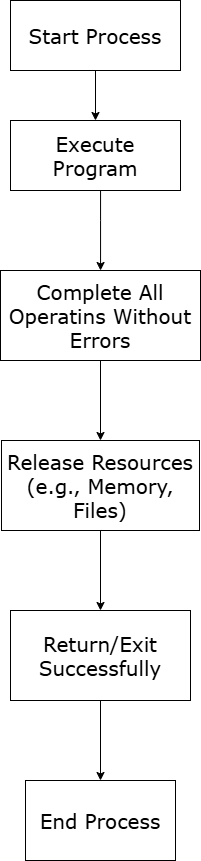
\includegraphics[width=0.2\linewidth]{Normal.png}
        \caption{Normal Termination}
        \label{fig:enter-label}
    \end{figure}
    
        \begin{itemize}
            Proses Normal Termination adalah suatu kondisi di mana sebuah proses menyelesaikan fungsinya yang dimaksudkan tanpa mengalami kesalahan atau pengecualian. Ini adalah akhir eksekusi proses yang terkontrol dan disengaja. Dalam kode program, biasanya ada instruksi atau statement yang menunjukkan akhir dari proses, seperti return di fungsi main dalam bahasa C atau Java. Proses ini adalah bagian dari siklus hidup normal sebuah proses.
        \end{itemize}
    
        Skenario umum untuk terminasi normal:
        \begin{itemize} 
            \item Penyelesaian proses: Proses telah menyelesaikan semua tugasnya dan mencapai titik akhir alami.
            \item Terminasi yang diinisiasi oleh pengguna: Pengguna telah secara eksplisit meminta proses untuk berhenti, biasanya melalui perintah atau antarmuka.
            \item Pengembalian dari fungsi: Sebuah proses dapat terminasi ketika sebuah fungsi yang dijalankan mengembalikan nilai yang mengindikasikan penyelesaian.
        \end{itemize}
    
        Karakteristik terminasi normal:
        \begin{itemize} 
            \item Proses terminasi dengan cara yang dapat diprediksi dan teratur.
            \item Tidak ada masalah atau pengecualian yang tidak terduga yang menyebabkan proses berakhir sebelum waktunya.
            \item Proses melepaskan semua sumber daya yang digunakannya (misalnya, memori, file, koneksi jaringan) sebelum terminasi.
        \end{itemize}
        
        Contoh terminasi normal:
        \begin{itemize}
            \item Sebuah proses browser web menyelesaikan pemuatan halaman web.
            \item Sebuah proses editor teks menyimpan dokumen dan kemudian keluar.
            \item Sebuah tugas latar belakang menyelesaikan pekerjaannya yang dijadwalkan dan terminasi.
        \end{itemize} 
    
    
    \item 
    \subsubsection {Abnormal Termination}
    
    \item Abnormal Termination adalah Proses berakhir tidak normal akibat adanya kesalahan yang tidak dapat ditangani dengan benar. Hal ini sering kali disebabkan oleh kondisi yang tidak diharapkan yang membuat proses tidak dapat melanjutkan eksekusi
    
        \begin{figure}
            \centering
            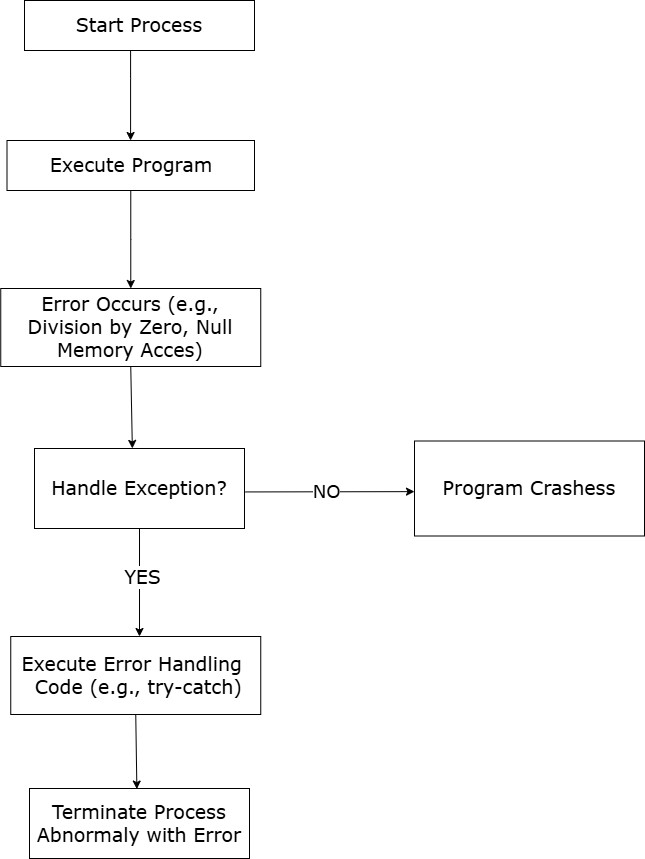
\includegraphics[width=0.5\linewidth]{Abnormal.png}
            \caption{Abnormal Termination}
            \label{Abnormal}
        \end{figure}
    
    
    Penyebab Terminasi Abnormal:
    \begin{itemize}
        \item Kesalahan Logika: Kesalahan dalam kode program, seperti pembagian dengan nol, akses array di luar batas, atau penggunaan pointer yang tidak valid.
        \item Kehabisan Sumber Daya: Proses kehabisan sumber daya yang dibutuhkan untuk beroperasi, seperti memori, file descriptor, atau waktu CPU.
        \item Sinyal: Proses menerima sinyal yang memaksanya untuk berhenti, seperti sinyal SIGKILL (terminate immediately) atau SIGSEGV (segmentation fault).
        \item Kesalahan Perangkat Keras: Kerusakan perangkat keras dapat menyebabkan proses berhenti secara tiba-tiba.
        \item Deadlock: Dua atau lebih proses saling menunggu satu sama lain, sehingga tidak ada yang dapat melanjutkan eksekusi.
        \item Interupsi: Terjadinya interupsi yang tidak dapat ditangani oleh sistem operasi.
    \end{itemize}
    
        Kontras dengan terminasi abnormal:
        \begin{itemize}
            \item Terminasi abnormal terjadi ketika sebuah proses berakhir secara tidak terduga karena kesalahan, pengecualian, atau keadaan tak terduga lainnya. Hal ini dapat menyebabkan perilaku yang tidak terkendali, kebocoran sumber daya, atau ketidakstabilan sistem.
        \end{itemize}
    
    Dampak Terminasi Abnormal :
    \begin{itemize}
        \item Kehilangan Data: Data yang sedang diproses oleh proses yang terminasi secara abnormal mungkin hilang atau rusak.
        \item Ketidakstabilan Sistem: Terminasi abnormal dapat menyebabkan sistem menjadi tidak stabil atau bahkan crash.
        \item Kerusakan Data: Data yang disimpan di disk atau memori dapat rusak jika proses tidak sempat menyimpan data dengan benar sebelum terminasi.
        \item Gangguan Proses Lain: Terminasi abnormal suatu proses dapat mempengaruhi proses lain yang berinteraksi dengannya.
    \end{itemize}
    
    
    Mekanisme Penanganan Terminasi Abnormal:
    \begin{itemize}
        Sistem Operasi: Sistem operasi akan berusaha untuk mendeteksi dan menangani terminasi abnormal. Ini melibatkan mekanisme seperti:
    \end{itemize}
    
    
        \begin{itemize}
            \item Penanganan Pengecualian: Sistem operasi akan menangkap pengecualian yang terjadi selama eksekusi proses dan mengambil tindakan yang sesuai, seperti menghentikan proses atau menampilkan pesan kesalahan.
            \item Pengawasan Memori: Sistem operasi akan memantau penggunaan memori oleh proses untuk mencegah terjadinya akses memori yang tidak sah.
            \item Pengawasan Waktu: Sistem operasi akan membatasi waktu eksekusi suatu proses untuk mencegah proses berjalan terlalu lama dan menghabiskan sumber daya sistem.
            \item     Debugging: Pengembang dapat menggunakan debugger untuk melacak kesalahan yang menyebabkan terminasi abnormal dan memperbaiki kode program.
        \end{itemize}
    
    
    Contoh Terminasi Abnormal
    \begin{itemize}
        \item Program crash: Sebuah program tiba-tiba berhenti bekerja dan menampilkan pesan kesalahan.
        \item Blue Screen of Death (BSOD): Sistem operasi Windows mengalami kegagalan fatal dan menampilkan layar biru.
        \item Kernel panic: Sistem operasi Linux mengalami kegagalan yang sangat serius dan tidak dapat melanjutkan operasi.
    \end{itemize}
    
    
    
    Pencegahan Terminasi Abnormal:
    \begin{itemize}
        \item Pengujian yang Memadai: Melakukan pengujian yang menyeluruh pada perangkat lunak untuk menemukan dan memperbaiki bug sebelum di-deploy.
        \item Penanganan Pengecualian: Menulis kode yang dapat menangani berbagai jenis pengecualian yang mungkin terjadi.
        \item Manajemen Memori yang Baik: Memastikan alokasi dan dealokasi memori dilakukan dengan benar untuk mencegah kebocoran memori.
        \item Validasi Input: Memeriksa semua input pengguna untuk memastikan bahwa input tersebut valid dan tidak akan menyebabkan kesalahan.
    \end{itemize}
    
    \begin{itemize}
    \item {Wahab, A., & Mubarok, R. (2019). Pengenalan Sistem Operasi (Edisi Revisi). Penerbit Andi.}
    \item {Hidayat, M., & Santoso, A. (2018). "Analisis Penanganan Error dan Exception Handling Pada Bahasa Pemrograman Java." Jurnal Ilmu Komputer dan Teknologi Informasi, 5(1), 55-62.}
    \end{itemize}

\end{itemize}

\subsection{Introduction to Threads}
This section introduces the concept of threads and their relation to processes, covering:
\begin{itemize}
    \item Single-threaded vs. multi-threaded processes
    \item Benefits of multithreading
\end{itemize}

\begin{figure}[h]
    \centering
    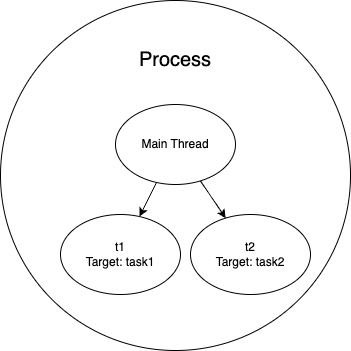
\includegraphics[width=0.5\textwidth]{/Users/khawaritzmi/Unhas/os_report_mid2024/b_class/asset/example.png}  % Sesuaikan nama file dan ukurannya
    \caption{Ini adalah gambar contoh dari multithreading.}
    \label{fig:contoh_gambar}
\end{figure}

Seperti yang terlihat pada Gambar \ref{fig:contoh_gambar}, inilah cara menambahkan gambar dengan keterangan.

\subsection{File Systems}
File systems provide a way for the operating system to store, retrieve, and manage data. This section explains:
\begin{itemize}
    \item File system structure
    \item File access methods
    \item Directory management
\end{itemize}

\subsection{Input and Output Management}
Input and output management is key for handling the interaction between the system and external devices. This section includes:
\begin{itemize}
    \item Device drivers
    \item I/O scheduling
\end{itemize}

\subsection{Deadlock Introduction and Prevention}
Explores the concept of deadlocks and methods for preventing them:
\begin{itemize}
    \item Deadlock conditions
    \item Deadlock prevention techniques
\end{itemize}

\subsection{User Interface Management}
This section discusses the role of the operating system in managing the user interface. Topics covered include:
\begin{itemize}
    \item Graphical User Interface (GUI)
    \item Command-Line Interface (CLI)
    \item Interaction between the user and the operating system
\end{itemize}

\subsection{Virtualization in Operating Systems}
Virtualization allows multiple operating systems to run concurrently on a single physical machine. This section explores:
\begin{itemize}
    \item Concept of virtualization
    \item Hypervisors and their types
    \item Benefits of virtualization in modern computing
\end{itemize}

\section{Assignments and Practical Work}
\subsection{Assignment 1: Process Scheduling}
Students were tasked with implementing various process scheduling algorithms (e.g., FCFS, SJN, and RR) and comparing their performance under different conditions.
\subsubsection{Group 1}
\begin{python}
    class Process:
    def __init__(self, pid, arrival_time, burst_time):
        self.pid = pid
        self.arrival_time = arrival_time
        self.burst_time = burst_time
        self.completion_time = 0
        self.turnaround_time = 0
        self.waiting_time = 0
\end{python}

\begin{table}[htbp] % Optional: For floating position
    \centering
    \begin{tabular}{|c|c|c|} % Defines number of columns and alignment (c = center, l = left, r = right). '|' creates vertical lines.
    \hline
    Header 1 & Header 2 & Header 3 \\ % Column headers
    \hline
    Row 1, Column 1 & Row 1, Column 2 & Row 1, Column 3 \\ % First row of data
    \hline
    Row 2, Column 1 & Row 2, Column 2 & Row 2, Column 3 \\ % Second row of data
    \hline
    \end{tabular}
    \caption{Your table caption} % Optional: For adding a caption
    \label{tab:your_label} % Optional: For cross-referencing the table
\end{table}

\subsection{Assignment 2: Deadlock Handling}
In this assignment, students were asked to simulate different deadlock scenarios and explore various prevention methods.

\subsection{Assignment 3: Multithreading and Amdahl's Law}
This assignment involved designing a multithreading scenario to solve a computationally intensive problem. Students then applied **Amdahl's Law** to calculate the theoretical speedup of the program as the number of threads increased.

\subsection{Assignment 4: Simple Command-Line Interface (CLI) for User Interface Management}
Students were tasked with creating a simple **CLI** for user interface management. The CLI should support basic commands such as file manipulation (creating, listing, and deleting files), process management, and system status reporting.

\subsection{Assignment 5: File System Access}
In this assignment, students implemented file system access routines, including:
\begin{itemize}
    \item File creation and deletion
    \item Reading from and writing to files
    \item Navigating directories and managing file permissions
\end{itemize}

\section{Conclusion}
The first half of the course introduced core operating system concepts, including process management, scheduling, multithreading, and file system access. These topics provided a foundation for more advanced topics to be covered in the second half of the course.

\end{document}